\chapter{Resultados}\label{cap:resultados}

Se presentan los resultados del estudio empírico (4.470 ejecuciones en paralelo y 236 en serie, sin ningún fallo), siguiendo las cinco preguntas del capítulo~\ref{cap:intro}. Los tiempos absolutos dependen del equipo; interesan sobre todo
las proporciones y el crecimiento con el número de ciudades.

\section{Validación: los algoritmos exactos coinciden}

Fuerza bruta, Held--Karp y DFJ dan exactamente el mismo coste en todas las instancias en las que se pueden comparar: \textbf{234 instancias} (fuerza bruta frente a DFJ) y \textbf{280} (Held--Karp frente a DFJ), con cero discrepancias. Ninguna heurística devuelve un coste
inferior al óptimo. Este resultado respalda tanto la corrección de las tres implementaciones, que son muy distintas entre sí (enumeración, programación dinámica y programación entera), como el uso de DFJ como referencia del óptimo.

\section{Complejidad: tiempo y memoria frente al tamaño}\label{sec:complejidad}

Las figuras~\ref{fig:tiempo} y~\ref{fig:memoria} muestran, con el eje vertical logarítmico, cómo crecen el tiempo y la memoria con el número de ciudades (estudio B, grafo dirigido, mediana de las instancias; medido en serie). En escala logarítmica, una recta ascendente indica crecimiento
exponencial y una curva que se aplana, crecimiento polinómico.

\begin{figure}[htbp]
  \centering
  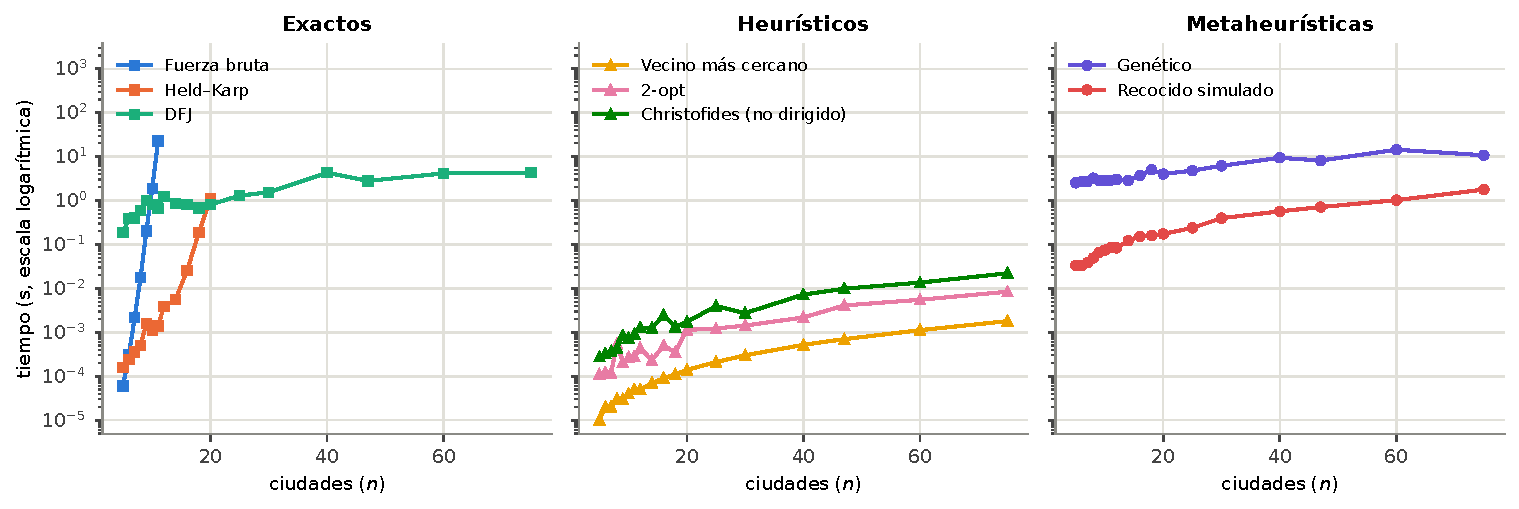
\includegraphics[width=\linewidth]{curvas_tiempo.pdf}
  \caption{Tiempo de cálculo frente al número de ciudades (escala logarítmica en el eje vertical). La fuerza bruta y Held--Karp se detienen en sus límites (11 y 20 ciudades).}
  \label{fig:tiempo}
\end{figure}

\begin{figure}[htbp]
  \centering
  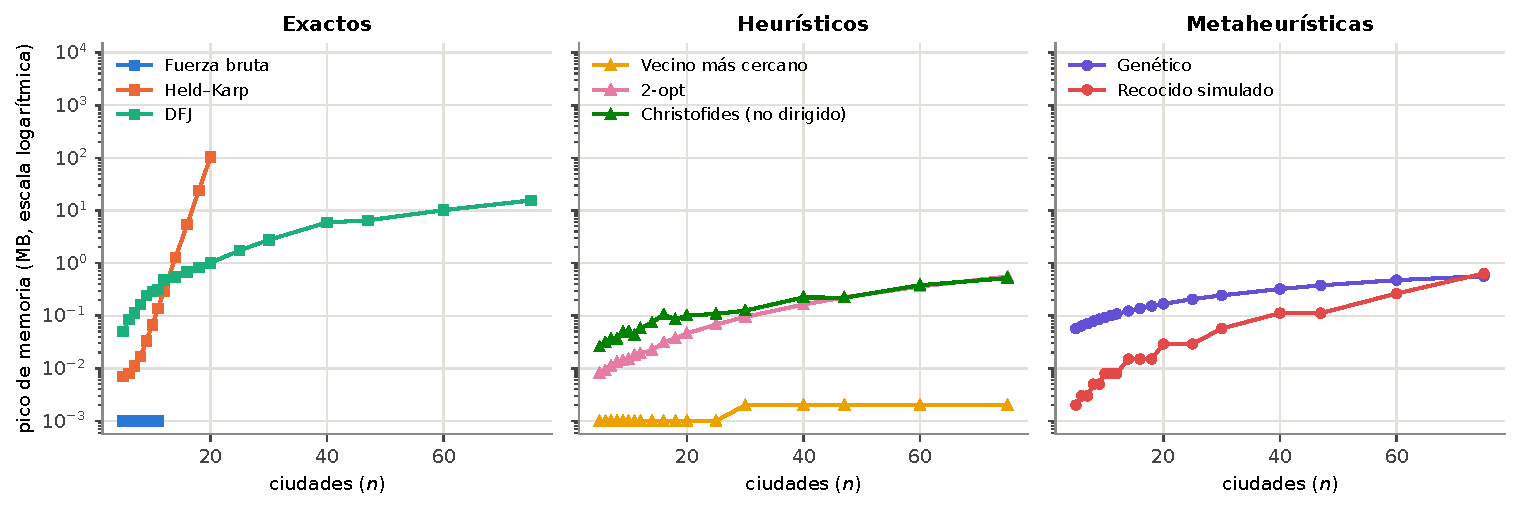
\includegraphics[width=\linewidth]{curvas_memoria.pdf}
  \caption{Pico de memoria reservada por Python frente al número de ciudades. La memoria de Held--Karp se duplica con cada ciudad.}
  \label{fig:memoria}
\end{figure}

\subsection{Complejidad en notación $O$: teoría frente a observación}

Para contrastar la complejidad teórica con la observada se ajustan los tiempos y la memoria medidos: un crecimiento exponencial $t\approx a\,b^{n}$ para los dos algoritmos de enumeración (donde $b$ es el factor por ciudad añadida) y una ley de potencias $t\approx a\,n^{k}$ para los demás
(ajuste lineal en escala logarítmica). El resultado se expresa en notación $O$ en la tabla~\ref{tab:bigo}.

\begin{table}[htbp]
  \centering
  \caption{Complejidad teórica y observada en notación $O$.}\label{tab:bigo}
  \footnotesize
  \begin{tabularx}{\linewidth}{@{}l X l X l@{}}
    \toprule
    Algoritmo & Tiempo (teoría) & Tiempo (observado) & Memoria (teoría) & Memoria (observada) \\
    \midrule
    Fuerza bruta & $O((n-1)!\cdot n)$ & $O(10{,}6^{\,n})$ & $O(n)$ & $\approx$ constante \\
    Held--Karp & $O(n^2\cdot 2^n)$ & $O(2{,}1^{\,n})$ & $O(n\cdot 2^n)$ & $O(2{,}1^{\,n})$ \\
    DFJ & $O(2^n)$ (peor caso) & $O(n)$ & $O(n^2)$ en la práctica & $O(n^{2})$ \\
    Vecino más cercano & $O(n^2)$ & $O(n^{1{,}9})$ & $O(n)$ & $\approx$ constante \\
    2-opt & $O(n^3)$ & $O(n^{1{,}8})$ & $O(n^2)$ & $O(n^{1{,}8})$ \\
    Christofides & $O(n^3)$ & $O(n^{1{,}6})$ & $O(n^2)$ & $O(n^{1{,}1})$ \\
    Recocido simulado & entre $O(n)$ y $O(n^2)$ & $O(n^{1{,}5})$ & $O(n^2)$ & $O(n^{2{,}1})$ \\
    Genético & $O(G\cdot P\cdot n\cdot q)$ & $O(n^{0{,}9})$ & $O(P\cdot n)$ & $O(n^{0{,}9})$ \\
    \bottomrule
  \end{tabularx}
\end{table}

Los dos algoritmos exactos de enumeración crecen de forma \textbf{exponencial}, en consonancia con la teoría: la fuerza bruta multiplica su tiempo por 10,6 con cada ciudad añadida ($R^2=1{,}00$; la teoría dice ``por $n$'', es decir, entre 9 y 11 en este rango) y Held--Karp por 2,1 ($R^2=0{,}96$; la
teoría dice aproximadamente 2), con una memoria que también se duplica por ciudad. El resto de algoritmos son \textbf{polinómicos}. El vecino más cercano ($n^{1,9}$) y el genético ($n^{0,9}$, lineal en $n$ por generación) coinciden con lo esperado; el 2-opt y Christofides salen con exponentes
menores que los teóricos, porque con 5 a 75 ciudades pesan los costes fijos y las operaciones vectorizadas de NumPy, y el exponente teórico se refiere al peor caso. DFJ es el caso más llamativo: su peor caso es exponencial, pero en estas instancias el tiempo crece apenas
de forma lineal (de 0,2~s con 5 ciudades a 4,3~s con 75).

Conviene recordar que la $O$ observada es una \emph{estimación} con tamaños de 5 a 75 ciudades y no una demostración.

\section{De enumerar a ser inteligente: la mejora entre algoritmos exactos}

La tabla~\ref{tab:exactos} compara el tiempo necesario para resolver al óptimo una instancia de $n$ ciudades con los tres algoritmos exactos (serie, grafo dirigido).

\begin{table}[htbp]
  \centering
  \caption{Tiempo (s) para resolver al óptimo una instancia de $n$ ciudades. «--» indica que el algoritmo no es aplicable.}\label{tab:exactos}
  \small
  \begin{tabular}{@{}r r r r@{\qquad}r r@{}}
    \toprule
    $n$ & Fuerza bruta & Held--Karp & DFJ & FB\,/\,HK & DFJ\,/\,HK \\
    \midrule
    8  & 0,018 & 0,0005 & 0,59 & 36 & 1.184 \\
    10 & 1,87 & 0,0011 & 0,82 & 1.641 & 747 \\
    11 & 22,5 & 0,0014 & 0,66 & 16.047 & 469 \\
    12 & -- & 0,0038 & 1,25 & -- & 328 \\
    14 & -- & 0,0056 & 0,85 & -- & 152 \\
    16 & -- & 0,026 & 0,82 & -- & 31,5 \\
    18 & -- & 0,18 & 0,68 & -- & 3,7 \\
    20 & -- & 1,10 & 0,81 & -- & 0,73 \\
    30 & -- & -- & 1,55 & -- & -- \\
    47 & -- & -- & 2,80 & -- & -- \\
    75 & -- & -- & 4,31 & -- & -- \\
    \bottomrule
  \end{tabular}
\end{table}

Held--Karp es \textbf{36 veces más rápido} que la fuerza bruta con 8 ciudades, \textbf{1.600 veces} con 10 y \textbf{16.000 veces} con 11. DFJ, en cambio, es \emph{más lento} que Held--Karp con pocas ciudades (el arranque del \emph{solver} cuesta entre 0,2 y 1~s: con 11 ciudades es 469 veces
más lento), pero \textbf{no tiene su pared}: las curvas se cruzan hacia las \textbf{20 ciudades} (0,81~s de DFJ frente a 1,10~s de Held--Karp), y DFJ resuelve 75 ciudades al óptimo en 4,3~s. En resumen: de 5 a 7 ciudades cualquiera sirve; de 8 a 19, Held--Karp; \textbf{desde 20, DFJ}.

\section{Calidad: cuánto se aleja del óptimo lo que no lo garantiza}

La tabla~\ref{tab:calidad} y la figura~\ref{fig:desviacion} muestran la desviación media respecto al óptimo de los algoritmos no exactos (estudio B; media de los subconjuntos y las semillas).

\begin{table}[htbp]
  \centering
  \caption{Desviación media respecto al óptimo (\%), por número de ciudades. Grafo dirigido, salvo Christofides (no dirigido).}\label{tab:calidad}
  \small
  \begin{tabular}{@{}r r r r r r@{}}
    \toprule
    $n$ & Vecino más cercano & Christofides & 2-opt & Recocido & Genético \\
    \midrule
    11 & 8,0 & 7,6 & 0,4 & 0,0 & 0,0 \\
    20 & 20,9 & 5,3 & 1,1 & 0,1 & 1,4 \\
    47 & 30,4 & 14,6 & 1,1 & 2,3 & 5,0 \\
    75 & 31,8 & 13,6 & 4,5 & 4,4 & 6,1 \\
    \bottomrule
  \end{tabular}
\end{table}

\begin{figure}[htbp]
  \centering
  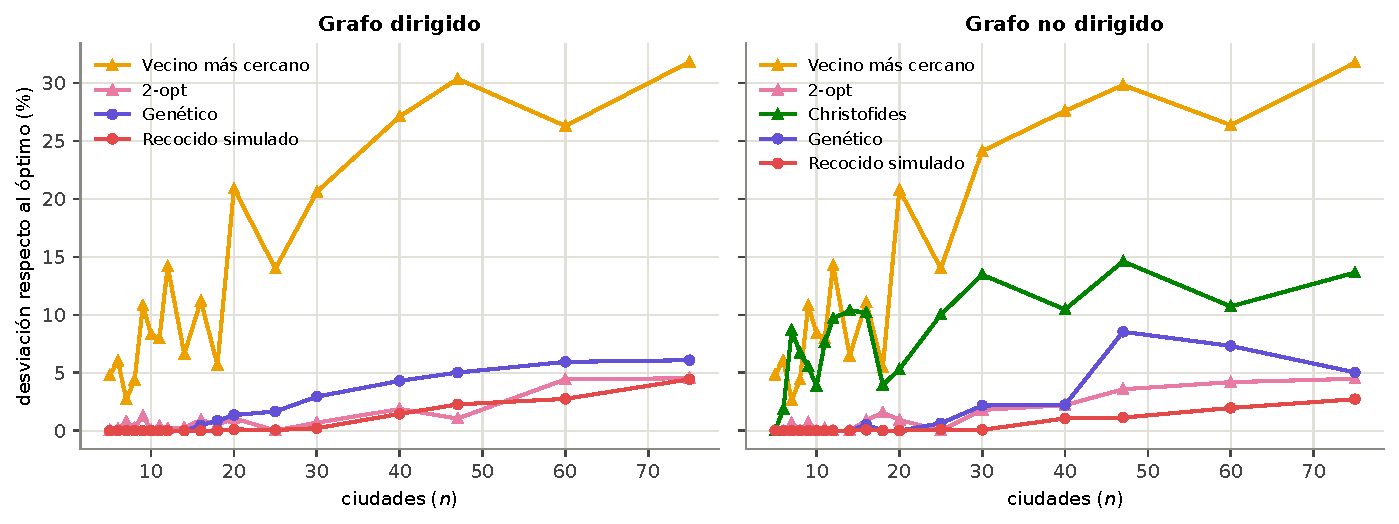
\includegraphics[width=0.92\linewidth]{desviacion.pdf}
  \caption{Desviación media respecto al óptimo (\%) en función del número de ciudades, en el grafo dirigido (izquierda) y no dirigido (derecha).}
  \label{fig:desviacion}
\end{figure}

\begin{itemize}
  \item El \textbf{vecino más cercano} es siempre el peor (entre un 3~\% y un 32~\% por encima del óptimo de media, hasta un 42~\% en un caso concreto) y empeora con el tamaño: solo sirve como punto de partida.
  \item \textbf{Christofides} cumple siempre su garantía (peor caso individual medido: +19,7~\%, muy por debajo del 50~\%), pero queda por encima del 2-opt: la garantía es un peor caso, no una predicción.
  \item El \textbf{2-opt} es el mejor equilibrio: con un error del 1--5~\% tarda milisegundos.
  \item \textbf{Recocido y genético llegan al óptimo hasta unas 14 ciudades} y después se alejan poco a poco. No mejoran al 2-opt en estos tamaños y tardan entre 170 y 2.000 veces más.
\end{itemize}

\subsection{Variabilidad de los algoritmos con azar}

Un solo resultado no describe a un algoritmo estocástico. Con 47 ciudades, el genético va del 1,0~\% al 8,3~\% de desviación (mediana 5,2~\%) y el recocido del 0,0~\% al 6,6~\% (mediana 2,2~\%); la figura~\ref{fig:dispersion} muestra cada ejecución.
Las medias esconden además casos malos: en la peor versión de toda España, el 2-opt llega a +18~\%, el recocido a +26~\% y el genético a +49~\%.

\begin{figure}[htbp]
  \centering
  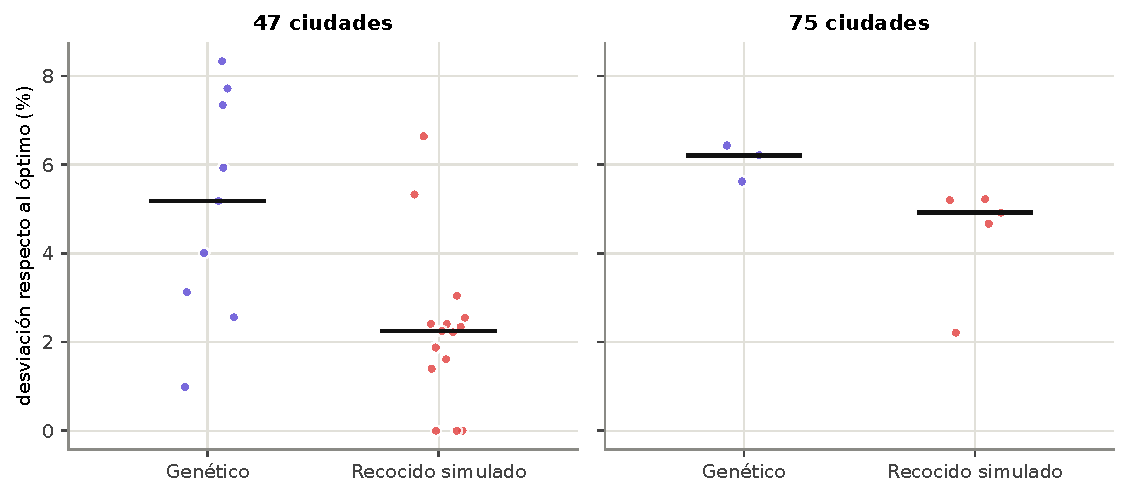
\includegraphics[width=0.7\linewidth]{dispersion.pdf}
  \caption{Desviación de cada ejecución del genético y del recocido simulado (grafo dirigido). La raya negra es la mediana.}
  \label{fig:dispersion}
\end{figure}

\section{Efecto de la versión del grafo}\label{sec:versiones_resultados}

Los resultados dependen tanto de la versión como del algoritmo. La figura~\ref{fig:rutas} muestra, para las 47 capitales, tres rutas sobre las carreteras reales.

\begin{figure}[htbp]
  \centering
  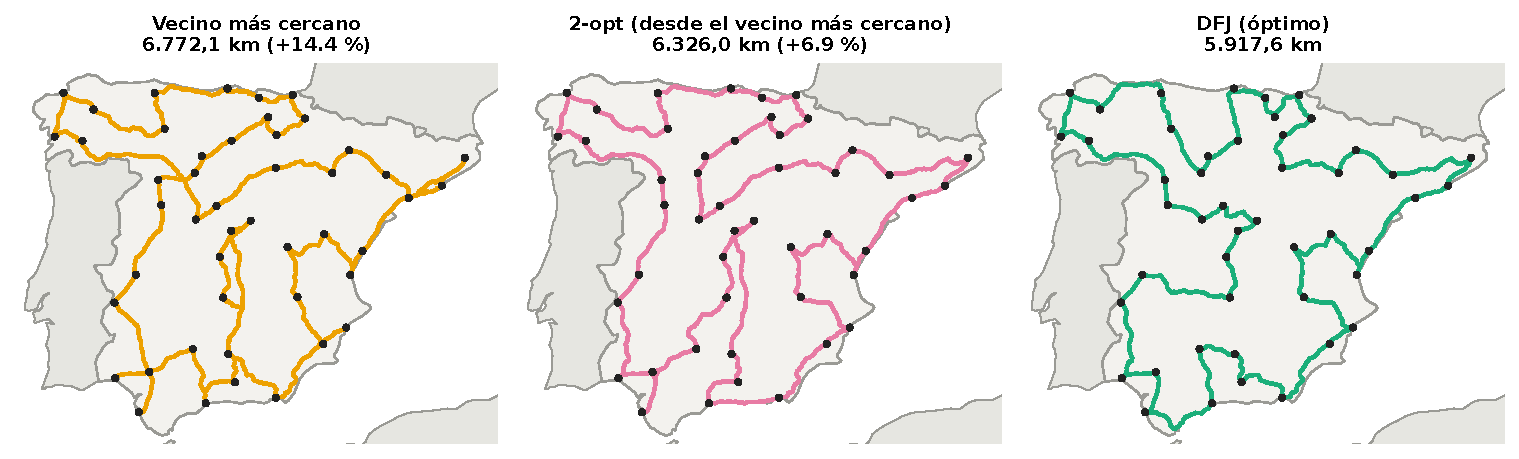
\includegraphics[width=\linewidth]{rutas_47.pdf}
  \caption{Rutas de las 47 capitales (versión \texttt{completo}/km, con sentidos únicos, saliendo de Madrid): vecino más cercano, 2-opt y óptimo (DFJ), dibujadas sobre el trazado de las carreteras.}
  \label{fig:rutas}
\end{figure}

\paragraph{Red de carreteras.} La tabla~\ref{tab:optimos} da el óptimo en cada versión de toda España. Sin autovías el óptimo cuesta un \textbf{30--38~\% más de kilómetros y casi el doble de tiempo} (+99~\% a +108~\%); con
\texttt{autovias\_principales}, solo un 3--4~\% más. Con \texttt{solo\_autovias} cuesta un 32--38~\% más de kilómetros y quedan fuera tres ciudades.

\paragraph{Sentido de las vías.} Ignorar los sentidos únicos apenas cambia el óptimo en la mayoría de las redes (0,7--4,0~\%), pero en \texttt{solo\_autovias} los sentidos cuestan un \textbf{13--19~\%}, porque en una red solo de autovías no se puede dar la vuelta.
Los heurísticos lo notan: con grafo dirigido el 2-opt se aleja de media un 6,9~\% (2,6~\% en no dirigido), el genético un 10,6~\% (4,3~\%) y el recocido un 5,2~\% (2,3~\%).

\paragraph{Calidad de los heurísticos según la red.} La tabla~\ref{tab:gapred} muestra la desviación media por red. \texttt{solo\_autovias} es la más difícil para los heurísticos (2-opt 8,1~\%, recocido 6,7~\%, genético 13,4~\%) y \texttt{sin\_autovias}, la mejor para el 2-opt (1,8~\%).

\begin{table}[htbp]
  \centering
  \caption{Óptimo (DFJ) en las versiones de toda España y coste respecto a la red completa (47 y 75 ciudades; con 44 y 72 en \texttt{solo\_autovias}).}\label{tab:optimos}
  \footnotesize
  \begin{tabular}{@{}l c r r r r@{}}
    \toprule
    & & \multicolumn{2}{c}{Óptimo en km} & \multicolumn{2}{c}{Óptimo en horas} \\
    \cmidrule(lr){3-4}\cmidrule(lr){5-6}
    Red & Ciudades & dirigido & no dirigido & dirigido & no dirigido \\
    \midrule
    \texttt{completo} & 47 & 5.917,6 & 5.875,3 & 63,3 & 62,2 \\
    & 75 & 6.146,2 & 6.069,8 & 67,7 & 65,9 \\
    \texttt{autovias\_principales} & 47 & 6.094,7 & 6.054,0 & 64,7 & 63,5 \\
    & 75 & 6.377,5 & 6.242,6 & 69,8 & 67,1 \\
    \texttt{sin\_autovias} & 47 & 7.661,4 & 7.573,7 & 125,7 & 123,8 \\
    & 75 & 8.465,7 & 8.331,4 & 140,6 & 137,4 \\
    \texttt{solo\_autovias} & 44 / 47 & 7.814,1 & 6.900,1 & 70,1 & 61,3 \\
    & 72 / 75 & 8.509,3 & 7.222,6 & 76,5 & 64,6 \\
    \bottomrule
  \end{tabular}
\end{table}

\begin{table}[htbp]
  \centering
  \caption{Desviación media (\%) de cada algoritmo en las 32 versiones de toda España, según la red de carreteras.}\label{tab:gapred}
  \small
  \begin{tabular}{@{}l r r r r@{}}
    \toprule
    Algoritmo & \texttt{completo} & \texttt{autovias\_principales} & \texttt{sin\_autovias} & \texttt{solo\_autovias} \\
    \midrule
    Vecino más cercano & 19,7 & 26,3 & 30,8 & 23,4 \\
    Christofides & 12,1 & 12,6 & 13,9 & 11,5 \\
    2-opt & 4,6 & 4,6 & 1,8 & 8,1 \\
    Recocido simulado & 2,9 & 2,7 & 2,7 & 6,7 \\
    Genético & 4,7 & 5,5 & 6,3 & 13,4 \\
    \bottomrule
  \end{tabular}
\end{table}

\paragraph{Kilómetros frente a tiempo.} La ruta más corta no es la más rápida. Para las 47 capitales, la ruta de mínimos kilómetros mide 5.917,6~km y tarda 64,5~h; la de mínimo tiempo mide 6.002,4~km y tarda 63,3~h. La ruta más rápida ahorra \textbf{1,2~h (1,9~\%)} a cambio de
\textbf{84,8~km (+1,4~\%)}, y las dos rutas comparten 31 de sus 47 tramos entre ciudades.

\section{Calidad frente a tiempo: ¿qué conviene usar?}

La figura~\ref{fig:calidad_tiempo} sitúa cada algoritmo según su tiempo (eje horizontal, logarítmico) y su desviación media (eje vertical): lo mejor está abajo y a la izquierda. Con 11 ciudades se comparan todos; con 75 los exactos de enumeración ya no caben.

\begin{figure}[htbp]
  \centering
  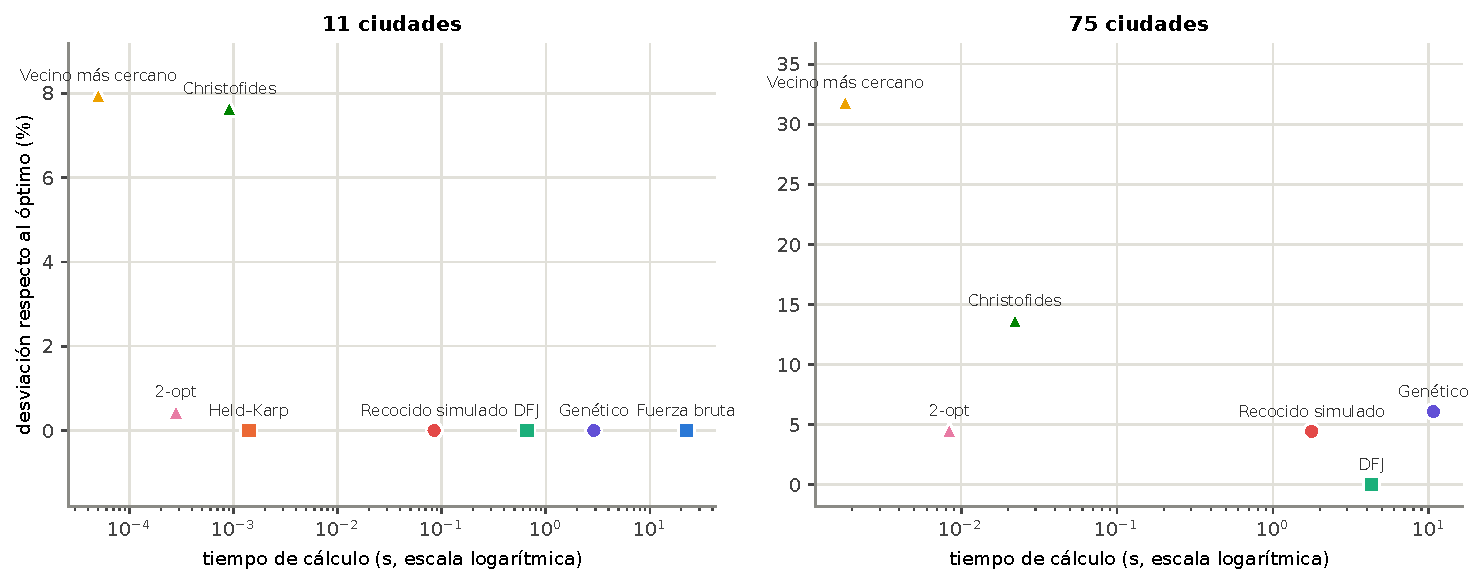
\includegraphics[width=\linewidth]{calidad_tiempo.pdf}
  \caption{Calidad frente a tiempo con 11 y con 75 ciudades (grafo dirigido; Christofides, no dirigido).}
  \label{fig:calidad_tiempo}
\end{figure}

\begin{table}[htbp]
  \centering
  \caption{Resumen con 47 y 75 ciudades (grafo dirigido): calidad, tiempo (serie) y memoria.}\label{tab:resumen}
  \small
  \begin{tabular}{@{}r l r r r r@{}}
    \toprule
    $n$ & Algoritmo & Desv. media (\%) & Peor (\%) & Tiempo (s) & Memoria (MB) \\
    \midrule
    47 & DFJ & 0,0 & 0,0 & 2,795 & 6,51 \\
    & 2-opt & 1,1 & 1,6 & 0,004 & 0,22 \\
    & Recocido simulado & 2,3 & 6,6 & 0,710 & 0,11 \\
    & Genético & 5,0 & 8,3 & 8,124 & 0,38 \\
    & Vecino más cercano & 30,4 & 36,1 & 0,001 & $<0{,}01$ \\
    \midrule
    75 & DFJ & 0,0 & 0,0 & 4,310 & 15,54 \\
    & Recocido simulado & 4,4 & 5,2 & 1,775 & 0,64 \\
    & 2-opt & 4,5 & 4,5 & 0,008 & 0,56 \\
    & Genético & 6,1 & 6,4 & 10,724 & 0,56 \\
    & Vecino más cercano & 31,8 & 31,8 & 0,002 & $<0{,}01$ \\
    \bottomrule
  \end{tabular}
\end{table}

\section{Cuánto distorsiona medir en paralelo}\label{sec:calibracion}

La calibración repitió en serie 15 tareas de la pasada en paralelo. El tiempo en paralelo resultó \textbf{2,46 veces mayor} de mediana, entre $\times 2{,}06$ (genético) y $\times 2{,}72$ (recocido simulado). Esto confirma que los tiempos solo son fiables en la pasada en serie, y justifica haber
medido los tiempos y la memoria de las curvas de complejidad en esa pasada.
